\PassOptionsToPackage{sols}{handout}
\documentclass[main]{subfiles}
\setcounterrefbeforedot{chapter}{m-ws1-4}
\setcounterrefafterdot{section}{m-ws1-4}
\addtocounter{section}{-1}
\usepackage{solutions}

\begin{document}

\section{Implicit Differentiation} \label{ws1-4}

% \begin{objectives}
% Learning Objectives:

% \begin{itemize}[topsep=0pt,partopsep=0pt,parsep=8pt,itemsep=0pt]

% \item You should understand that an equation involving two variables
%   describes a relationship between the two variables; graphically, we
%   visualize such a relationship as an implicit curve (for example,
%   $x^2+y^2=25$ defines an implicit curve in the $xy$-plane).

% \item You should recognize and be able to write the equation of a circle
%   centered at the origin with radius $r$. 

% \item You should be able to use implicit differentiation to find
%   $\frac{dy}{dx}$ given an equation involving $x$ and $y$.  (From Math Ma,
%   you should be able to represent this graphically or interpret it in the
%   context of a word problem.)

% \item You should be able to find the points on an implicit curve at which
%   the tangent line has a given slope.
% \end{itemize}
% \end{objectives}

\textbf{Key Idea}: Equations can implicitly define one variable as a function of another variable.

\begin{enumerate}

\item 
\begin{problem}
In Math Ma, we were almost always working with equations that looked like $y=f(x)$. When an equation is in this form, we say that it \emph{explicitly} defines $y$ as a function of $x$.

Does the equation $y-x^2=0$ explicitly define $y$ as a function of $x$? If not, can you rearrange the equation into an explicit formula?
\end{problem}
\pspace{\stretch{0.5}}

\begin{solution}
    The equation $y-x^2=0$ does not explicitly define $y$ as a function of $x$, because it's not in the form $y=f(x)$. We can rearrange the equation into the explicit formula $y=x^2$.
\end{solution}

\item The graph of $x=y^5+y$ is shown below, next to b). 

\begin{enumerate}
\item 
\begin{problem}
This equation \emph{explicitly} defines $x$ as a function of $y$. Let's call it $x=g(y)$. Find the value of $g(1)$.
\end{problem}
\pspace{\stretch{0.5}}

\begin{solution}
    $g(1)=1^5+1=\fbox{2}$
\end{solution}

\end{enumerate}

\begin{minipage}[t]{2.1in}\vspace{0pt}
    
\includegraphics[height=1.75in]{tikz/1-4/1-4-quintic.pdf}
\end{minipage}
\hfill
\begin{minipage}[t]{4in}\vspace{0pt}
\begin{enumerate}[start=2]
\item
\begin{problem}
It's very difficult to solve this equation for $y$ using algebra. But we can see graphically that $y$ is indeed a function of $x$. We say that the equation \emph{implicitly} defines $y$ as a function of $x$, and we call the function it defines an \emph{implicit function.} 

Let $y=f(x)$ be the implicit function defined by $x=y^5+y$. Find the value of $f(2)$.
\end{problem}

\begin{solution}
    Since $f(2)$ is the value of $y$ when $x=2$ and we know that the point $(2, 1)$ is on the graph, $f(2)=\fbox{1}$.
\end{solution}
\end{enumerate}
\end{minipage}

\item 
\begin{enumerate}
\item 
\begin{problem}
Sketch the graph of $x^2+y^2=25$.
\end{problem}
\pspace{\stretch{2}}

\begin{solution}
    \begin{center}
        \begin{tikzpicture}
            \begin{axis}[
            xlabel=$x$, ylabel=$y$,
            xmin=-7.5, xmax=7.5, ymin=-7.5, ymax=7.5,
            xtick={-5,5}, ytick={-5,5},
            axis equal image
            ]
                \addplot[domain=0:360] ({5*cos(x)},{5*sin(x)});
            \end{axis}
        \end{tikzpicture}
    \end{center}
\end{solution}


\item
\begin{problem}
To define a function from this equation, we need to ``erase'' part of the graph. We could erase either the top half or the bottom half. Each choice gives us a different implicit function defined by $x^2+y^2=25$. Find explicit formulas for  both functions.
\end{problem}
\pspace{\stretch{2}}

\begin{solution}
    Solving $x^2+y^2=25$ gives us:
    \begin{align*}
        x^2 + y^2 &= 25 \\
        y^2 &= 25 - x^2 \\
        y &= \pm \sqrt{25-x^2}
    \end{align*}
    The formula for the top half of the circle is \fbox{$y=\sqrt{25-x^2}$}. A formula for the bottom half of the circle is \fbox{$y=-\sqrt{25-x^2}$}.
\end{solution}

\end{enumerate}

\end{enumerate}

\pspace{\newpage}

\textbf{Key Idea}: We can use the Chain Rule to differentiate implicit functions without an explicit formula.

\begin{enumerate}[resume]
\item We're going to consider two methods for finding the slope of a tangent line to the graph of an equation. 
\begin{enumerate}
\item
\begin{problem}
Using one of the explicit formulas you found in the last problem, determine the slope of the line tangent to the graph of $x^2+y^2=25$ at the point $(4, -3)$.
\end{problem}
\pspace{\vfill}

\begin{solution}
    Since the point $(4, -3)$ is on the bottom half of the circle, we should use the formula $y=-\sqrt{25-x^2}$. To find the slope of the tangent line at this point, we want to find $\diff{y}{x}$.
    \begin{align*}
        \diff{y}{x} &= \diff*{\!\left[-\sqrt{25-x^2}\right]}{x} \\[4pt]
        &= -\tfrac{1}{2}(25-x^2)^{-1/2} \cdot (-2x) \\[4pt]
        &= \frac{x}{\sqrt{25-x^2}} \\
        \intertext{Plugging in $x=4$:}
        \diff{y}{x}[x=4] &= \frac{4}{\sqrt{25-4^2}} \\[4pt]
        &= \fbox{$\dfrac{4}{3}$}
    \end{align*}
\end{solution}

\item 
\begin{problem}
If we didn't have an explicit formula, we could still find $\diff{y}{x}$ at the point $(4,-3)$ by treating $y$ as an implicit function of $x$ and differentiating both sides of $x^2+y^2=25$ with respect to $x$. Try it.
\end{problem}
\pspace{\vfill}

\begin{solution}
    If we think of $y$ as a function of $x$, then
    \begin{align*}
        \diff*{\!\left[x^2+y^2\right]}{x} &= \diff*{25}{x} \\[4pt]
        2x + 2y\diff{y}{x} &= 0 \\[4pt]
        2y\diff{y}{x} &= -2x \\[4pt]
        \diff{y}{x} &= \frac{-x}{y}\\
        \intertext{Plugging in $x=4$ and $y=-3$:}
        \diff{y}{x}[(4,-3)] &= \fbox{$\dfrac{4}{3}$}
    \end{align*}
\end{solution}

\item
\begin{problem}
Which method did you like more?
\end{problem}
\pspace{\stretch{0.5}}

\begin{solution}
    The second method involves simpler calculations.
\end{solution}
\end{enumerate}

\end{enumerate}
\newpage

  \begin{framed}
    A curve defined by the graph of an equation is sometimes called an \emph{implicit curve.} Here are more examples.
    \begin{center} \vspace{-12pt}
      \begin{tabular}{ccc}
        
\includegraphics[width=\linewidth/3-\tabcolsep*2]{images/implicit-curve-heart}
        & 
\includegraphics[width=\linewidth/3-\tabcolsep*2]{images/implicit-curve-crooked-egg}
        & 
\includegraphics[width=\linewidth/3-\tabcolsep*2]{images/implicit-curve-trifolium.pdf}
        \vspace{2pt} \\
        & Crooked egg curve &  \\
        Heart curve & (a.k.a. lima bean) & Trifolium \vspace{2pt} \\
        $(x^2 + y^2 - 1)^3 - x^2 y^3 = 0$ & $(x^2 + y^2)^2 = x^3 + y^3$ &
        $(x^2 + y^2)^2 = 2 (x^3 - 3x y^2)$
      \end{tabular}  
    \end{center}
  \end{framed}

\begin{enumerate}[resume]
\item 
  \note{Historical Note: In 1638, Fermat and Descartes were both working
    on the problem of finding tangents to curves.  Descartes believed his
    method was better and came up with this curve as a ``challenge'' to
    Fermat.  Because the curve is implicitly defined, Descartes thought
    that Fermat would not be able to find tangent lines.  (Descartes
    himself could only find the tangent line at the ``vertex.'')  However,
    Fermat was able to find the tangent line at \textit{any} point on the
    curve.  (Reference:
    \url{http://www.jstor.org.ezp-prod1.hul.harvard.edu/stable/4145129}).

    Students tend to have trouble differentiating $\frac{9}{2} xy$ here;
    they may forget the Product Rule or throw in extra $\frac{dy}{dx}$
    terms.  }

  \begin{problem}[\stretch{0.75}]
    Find the equation for the tangent line to $x^3 + y^3 = \dfrac{9}{2}
    xy$, the \textit{folium of Descartes}, at the point $(1, 2)$.

    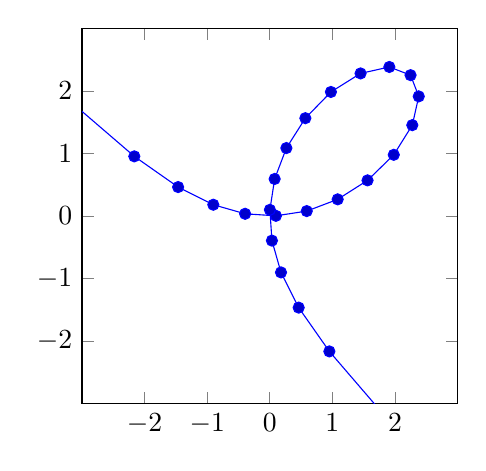
\begin{tikzpicture}
      \begin{axis}[axis equal=true, xmin=-3, xmax=3, ymin=-3, ymax=3,
        xtick={-2, -1, ..., 2}, ytick={-2, -1, ..., 2}, width=2.5in,
        height=2.5in] 
        \addplot+[domain=-30:120] ({9/2*sin(x)*cos(x)^2/(sin(x)^3+cos(x)^3)},
        {9/2*sin(x)^2*cos(x)/(sin(x)^3+cos(x)^3)});
      \end{axis}
    \end{tikzpicture}
  \end{problem}

  \begin{solution} 
    Let's start by finding the slope of the tangent line.  We know that
    the slope is just the value of $\frac{dy}{dx}$ at the point $(1, 2)$,
    so let's use implicit differentiation to find this slope (that looks
    simpler than trying to solve for $y$ in terms of $x$). 

    We start with the equation for the curve:
    \begin{align*}
      x^3 + y^3 &= \dfrac{9}{2}xy \\
      \intertext{Differentiate both sides with respect to $x$:} 
      \frac{d}{dx} \left( x^3 + y^3 \right) &=  \frac{d}{dx}
      \left(\fcolorbox{purple}{white}{$\displaystyle \frac{9}{2}$}\cdot
        \fcolorbox{green}{white}{$\displaystyle  x$}\cdot
        \fcolorbox{green}{white}{$\displaystyle  y$}\right) \\  
      3x^2 + 3y^2 \frac{dy}{dx} &= \frac{9}{2} \left( y + x
      \frac{dy}{dx} \right) \\
      \intertext{Plug in $x = 1, y = 2$:}
      3 + 12 \frac{dy}{dx} &= \frac{9}{2} \left( 2 + \frac{dy}{dx} \right)
      \\ 
      \shortintertext{Solve for $\frac{dy}{dx}$:}
      3 + 12 \frac{dy}{dx} &= 9 + \frac{9}{2} \frac{dy}{dx} \\
      \frac{15}{2} \frac{dy}{dx} &= 6 \\
      \frac{dy}{dx} &= \frac{4}{5}
    \end{align*}
    So, the line has slope $\dfrac{4}{5}$.  Since $(1, 2)$ is a point on
    the line, the equation of the line is $\boxed{y - 2 = \dfrac{4}{5} (x
      - 1)}$. 
  \end{solution}

  \pspace{\newpage}

\item 
  \note{The differentiation here is straightforward, but students may have
    trouble formulating a strategy for solving the problem.  Once they
    have solved it, ask them to go back to look at whether their answers seem
    reasonable to them given the picture.  (In particular, they may have
    found the point $(0, 0)$, but it's clear from the picture that this is
    not actually a correct answer to the question.)
    
    Matt note - I plan to draw attention to and contrast what we are given and what we are being asked in this problem vs the previous. Here we are given the slope as opposed to be asked to find the slope. This is a good plug for taking stock of what's given and asked before diving into work.}

\begin{enumerate}
\item
  \begin{problem}[\stretch{1}]
    Find the points at which the tangent line to the curve $y^2 = x^3 + 3x^2$ is horizontal. Be sure to check your answers with the graph.

    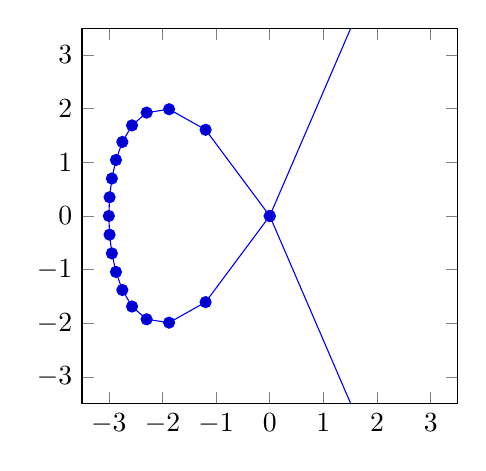
\begin{tikzpicture}
      \begin{axis}[axis equal=true, xmin=-3.5, xmax=3.5, ymin=-3.5,
        ymax=3.5, xtick={-3, -2, ..., 3}, ytick={-3, -2, ..., 3},
        width=2.5in, height=2.5in]        
        \addplot+[domain=-80:80] ({(-1-2*cos(2*x))/cos(x)^2},
        {(-1-2*cos(2*x))*sin(x)/cos(x)^3}); 
      \end{axis}
    \end{tikzpicture}    
  \end{problem}

  \begin{solution} 
    The question is asking us for points on the curve $y^2 = x^3 + 3x^2$
    where $\frac{dy}{dx} = 0$.  Graphically, we can see that there are two
    such points. To find their precise locations, let's use implicit
    differentiation to write an expression for $\frac{dy}{dx}$:
    \begin{align*}
      y^2 &= x^3 + 3x^2 \\
      \intertext{Differentiate both sides with respect to $x$:}
      2y\frac{dy}{dx} &= 3x^2 + 6x\\
      \intertext{We want $\frac{dy}{dx} = 0$, so let's just plug that in
        and see what it says:}
      0 &= 3x^2 + 6x \\
      \shortintertext{Now, we can solve for $x$:}
      0 &= 3x (x + 2) 
    \end{align*}
    So, $x = 0$ or $x = -2$.  Graphically, we can see that $x = 0$ is not
    actually a place where the tangent line is horizontal; in fact, the
    curve doesn't have a single tangent line at $x = 0$.

    On the other hand, $x = -2$ looks perfectly reasonable.  Let's find
    the corresponding $y$ values.  Since the curve has equation
    \begin{align*}
      y^2 &= x^3 + 3x^2, \\
      \shortintertext{when $x = -2$,}
      y^2 &= (-2)^3 + 3 (-2)^2 = 4,
    \end{align*}
    so $y = \pm 2$.  Therefore, the two points where the curve has a
    horizontal tangent line are \fbox{$(-2, 2)$ and $(-2, -2)$}.
    (Graphically, this looks right.)
  \end{solution}

\item
\begin{problem}
Find the points at which the slope of the tangent line to the graph is undefined. Be sure to check your answers with the graph.
\end{problem}
\pspace{\vfill}

\item
  \begin{problem}[\vfill]
    At what point(s) does
    the tangent line to the curve have slope $\frac{3}{2}$? 
  \end{problem}

  \begin{solution} 
    We can use basically the same strategy as in
    {{\#4}}.  We're looking for
    points on the curve $y^2 = x^3 + 3x^2$ where $\frac{dy}{dx} =
    \frac{3}{2}$.  As in {{\#4}},
    differentiating implicitly gives us
    \begin{align*}
      2y \frac{dy}{dx} &= 3x^2 + 6x \\
      \shortintertext{We want $\frac{dy}{dx} = \frac{3}{2}$, so we plug
        this in:} %
      3y &= 3x^2 + 6x \\
      y &= x^2 + 2x
    \end{align*}
    Unlike in {{\#4}}, we're not
    able to solve for $x$ yet.  However, if you look back at
    {{\#4}}, you see that we plugged
    back into the equation of the curve.  Let's do the same thing here;
    that is, we'll plug $y = x^2 + 2x$ into $y^2 = x^3 + 3x^2$:
    \begin{align*}
      (x^2 + 2x)^2 &= x^3 + 3x^2 \\
      x^4 + 4x^3 + 4x^2 &= x^3 + 3x^2 \\
      x^4 + 3x^3 + x^2 &= 0 \\
      x^2 (x^2 + 3x + 1) &= 0 \\
      x &= 0, \frac{-3 \pm \sqrt{5}}{2}
    \end{align*}
    We can see from the graph of the curve given in
    {{\#4}} that $x = 0$ is not
    really a solution, but the other two values of $x$ are solutions.  We
    can get the corresponding $y$-values from the fact that $y = x^2 +
    2x$, so the two points where the curve has slope $\frac{3}{2}$ are
    $\boxed{\left( \frac{-3 - \sqrt{5}}{2}, \frac{1 + \sqrt{5}}{2} \right)
      \text{ and } \left( \frac{-3 + \sqrt{5}}{2}, \frac{1 - \sqrt{5}}{2}
      \right)}$.  These two points are shown on the graph below:
    \begin{center}
      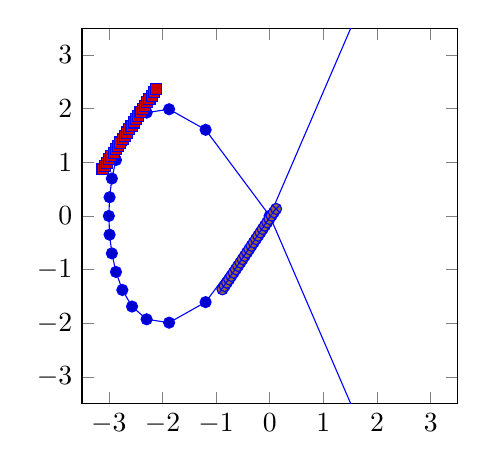
\begin{tikzpicture}
        \begin{axis}[axis equal=true, xmin=-3.5, xmax=3.5, ymin=-3.5,
          ymax=3.5, xtick={-3, -2, ..., 3}, ytick={-3, -2, ..., 3},
          width=2.5in, height=2.5in]        
          \addplot+[domain=-80:80] ({(-1-2*cos(2*x))/cos(x)^2},
          {(-1-2*cos(2*x))*sin(x)/cos(x)^3}); 
          \draw[red, fill=red] (axis cs: -2.618, 1.618) circle(1.5pt);
          \draw[red, fill=red] (axis cs: -0.382, -0.618) circle(1.5pt);
          \addplot+[blue, domain=-3.118:-2.118] {1.5*(x+2.618)+1.618};
          \addplot+[blue, domain=-0.882:0.118] {1.5*(x+0.382)-0.618};
        \end{axis}
      \end{tikzpicture}
    \end{center}
  \end{solution}

\end{enumerate}

\pspace{\newpage}

\item
    
  \begin{problem}
    Find the line tangent to the heart curve $(x^2 + y^2 - 1)^3 - x^2 y^3
    = 0$ at $(-1, 1)$.
  \end{problem}
    \pspace{\vfill}

  \begin{solution}    
    We start with the equation defining the curve.
    \begin{align*}
      (x^2 + y^2 - 1)^3 - x^2 y^3 &= 0 \\
      \intertext{Differentiate both sides with respect to $x$:}
      \frac{d}{dx} \left(\fcolorbox{red}{white}{$\displaystyle
          \fcolorbox{blue}{white}{$\displaystyle  \left(x^ { 2} + y^ { 2}
              -1\right)$}^ { 3} $}-
        \fcolorbox{green}{white}{$\displaystyle  x^ { 2} $}\cdot
        \fcolorbox{green}{white}{$\displaystyle  y^ { 3} $}\right) &=
      \frac{d}{dx} 0 \\
      3 \left(x^ { 2} + y^ { 2} -1\right)^ { 2} \cdot \frac{d}{dx}\left(x^
        { 2} + \fcolorbox{red}{white}{$\displaystyle \fcolorbox{blue}{white}{$\displaystyle  y$}^ { 2} $} -1\right)-\left[x^ { 2} \cdot \frac{d}{dx}
        \left(\fcolorbox{red}{white}{$\displaystyle
            \fcolorbox{blue}{white}{$\displaystyle  y$}^ { 3} $}\right)+
        2 x\cdot y^ { 3} \right] &= 0 \\
      3 (x^2 + y^2 - 1)^2 \left( 2x + 2y \frac{dy}{dx} \right) - x^2 \cdot
      3 y^2
      \frac{dy}{dx} - 2x y^3 &= 0 \\
      \intertext{Now, we can plug in $x = -1$,
        $y = 1$:}
      3 \left(-2 + 2 \frac{dy}{dx} \right) - 3 \frac{dy}{dx} +
      2 &= 0 \\
      3 \frac{dy}{dx} - 4 &= 0 \\
      \frac{dy}{dx} &= \frac{4}{3}
    \end{align*}
    Therefore, the slope of the tangent line is $\frac{4}{3}$, so the
    equation of the line is $\boxed{y - 1 = \frac{4}{3} (x + 1)}$.  (From
    the picture, we can see that the tangent line should indeed have
    positive slope.)
  \end{solution}


\item 
\begin{problem}
    WidgetCo sells widgets. The relationship between the price $p$ (in dollars) and quantity demanded $q$ (in thousands of units) for their widgets is $2p^2+2pq+q^2=800$. Currently, WidgetCo has priced their widgets at \$20, but nobody wants to buy any.
    Use implicit differentiation to approximate how many widgets WidgetCo will sell if they reduce the price by \$1. 
\end{problem}
\pspace{\vfill}

\begin{solution}
    To approximate the change in the quantity of widgets demanded due to a price change, we should find $\diff{q}{p}$, the instantaneous rate of change of the quantity with respect to price. We can use implicit differentiation to do this.
    \begin{align*}
        \diff*{\!\left[2p^2+2pq+q^2\right]}{p} &= \diff*{800}{p} \\[4pt]
        4p + \left(2q+2p\diff{q}{p}\right) + 2q\diff{q}{p} &= 0 \\[4pt]
        2p + q + p\diff{q}{p} + q\diff{q}{p} &= 0 \\[4pt]
        p\diff{q}{p} + q \diff{q}{p} &= -2p - q \\[4pt]
        \diff{q}{p} (p+q) &= -(2p+q) \\[4pt]
        \diff{q}{p} &= -\frac{2p+q}{p+q}
    \end{align*}
    We know that $p=20$, and since nobody wants to buy any widgets, $q=0$. So the current value of $\diff{q}{p}$ is 
    \begin{align*}
        \diff{q}{p} &= -\dfrac{2(20)+0}{20+0} \\[4pt]
        &= -2 \text{ units per dollar}
    \end{align*}
    This rate signifies that, for a small price change, the change in the quantity will be about $-2$ times as large as the change in the price. So if WidgetCo reduces the price by \$1, then the quantity demanded will go up by approximately 2 thousand units. Since WidgetCo is not currently selling any widgets, if they reduce the price by \$1, they will sell approximately \fbox{2 thousand widgets.}
\end{solution}

\end{enumerate}

\end{document}